\chapter{MARCO TEÓRICO}
\section{SISTEMAS DE CONDUCCIÓN AUTÓNOMA}
    Un sistema de conducción autónoma es una combinación de varios componentes o subsistemas donde las tareas de percepción, toma de decisiones y operación de un vehículo son desarrolladas por un sistema electrónico en lugar de un conductor humano
    \subsection{TAREAS DE LA CONDUCCIÓN AUTÓNOMA}
    Para lograr la conducción autónoma, se deben dividir tareas modulares, esto con el fin de poder realizar pruebas de cada componente y en caso de fallos, poder detectarlos aisladamente y que no afecten a los demás componentes.
    
    Las tareas son:
    \begin{itemize}[nosep]
        \item \textbf{Control lateral:} Control de la dirección o volante del vehículo.
        \item \textbf{Control longitudinal:} Control de la aceleración y freno.
        \item \textbf{Detección y respuesta de eventos y objetos:} (OEDR por sus siglas en inglés) detección de objetos importantes en la carretera como carriles y vehículos, también objetos fuera de la carretera como peatones o señales de tránsito. Como respuesta debe reaccionar a distintas situaciones peligrosas tanto deteniendo el coche o sacándolo de esa situación.
        \item \textbf{Planeamiento:} A corto plazo son las acciones inmediatas que debe tomar y modificar el camino ante adversidades, y a largo plazo es el mejor camino encontrado desde el origen al destino definido por el usuario.
    \end{itemize}
    estas están definidas en el documento de recomendaciones para vehículos autónomos de la Sociedad Internacional de Ingenieros de Automoción (SAE por sus siglas en inglés). \citep{J3016_201806}
    % \subsection{NIVELES DE AUTONOMÍA}
    % https://www.nhtsa.gov/technology-innovation/automated-vehicles-safety
    \subsection{ARQUITECTURA DE LA CONDUCCIÓN AUTÓNOMA}
    La arquitectura del software para la conducción autónoma se basa en una fase de adquisición de datos para entrenar los modelos predictivos y ajustar los algoritmos, y a partir de ahí una fase de inferencia, la cual tiene cuatro componentes principales:
    
    \begin{itemize}[nosep]
        \item \textbf{Percepción del ambiente:} Aquí se encuentran todos los modelos y algoritmos que nos permiten detectar objetos de interés a través de los sensores disponibles.
        \item \textbf{Mapeo del ambiente:} Una vez extraídos los objetos de interés, se procede a ubicarlos en posiciones relativas al vehículo.
        \item \textbf{Planificación de movimiento:} Se procede a armar un plan de acción para el estado del ambiente que se percibe en ese instante.
        \item \textbf{Control:} Una vez se realiza el plan de acción, se ejecuta enviando la información a los controladores de aceleración, freno y dirección.
    \end{itemize}
    
\section{VISIÓN COMPUTACIONAL}
    
    \subsection{PROCESAMIENTO DE IMÁGENES}
        Es la aplicación de operaciones del procesamiento de señales unidimensionales sobre imágenes, interpretadas como una señal bidimensional.
        \subsubsection{REPRESENTACIÓN DE IMÁGENES EN UNA COMPUTADORA}
        Una imágen $I$ está compuesta por píxeles $(x, y, v)$ cuyos componentes son una coordenada $(x, y) \in \mathbb{Z}^2$ y un valor $v \in \mathbb{Z}^c$, con $c$ el número de canales de color, siendo $c=1$ una imágen a escala de gristes y $c=3$ una imágen a colores Rojo, Verde y Azúl (RGB por sus siglas en inglés), definida sobre un conjunto $\Omega$. 
        
        \begin{equation}
            \Omega = \{(x, y)| 1 \leq x \leq N_{columnas} \land 1 \leq y \leq N_{filas}\} \subset \mathbb{Z}^2
        \end{equation}
        
        la representación que vemos en la computadora se le llama modelo grid cell, donde cada píxel es un cuadrado pequeño o celda con una intensidad de grises o canales RGB \citep{10.5555/2584519} con valores $0 \leq I_{x, y} \leq 255$.

        \begin{figure}[H]
            \centering
            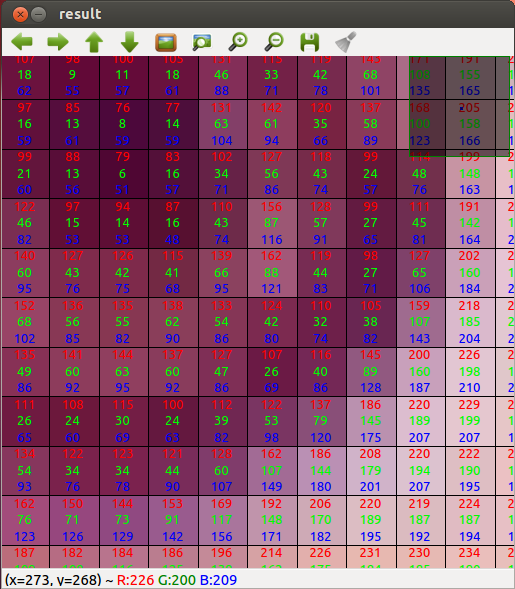
\includegraphics[scale=0.25]{imagenes/pixels}
            \caption{Intensidad de los canales de color RGB\\ Fuente: \citep{montabone_2012}}
        \end{figure}
        % \vspace{-8mm}
        % \begin{center}
        %     Fuente: \citep{montabone_2012}
        % \end{center}
        % \subsubsection{TRANSFORMACIONES DE PERSPECTIVA}
        % Page 359 birds eye
        % \subsubsection{DETECCIÓN DE BORDES}
        \subsubsection{CONVOLUCIÓN}
        Cuando deseamos aplicar alguna transformación de alguna imagen $I$ a alguna imagen $I'$ como difuminados, realce de bordes o extracción de alguna característica, debemos aplicar un operador local lineal entre un filtro que acentúe la característica en la imagen $I$.
        
        El filtro denotado por $W$ es una matriz cuadrada de dimensión $(2k+1) \times (2k+1)$, aplicada en forma de ventana deslizante sobre cada pedazo de la misma dimensión de la imagen original, siendo $(x, y)$ el punto central de cada sección sobre la que se opera, se define la convolución como:
        
        \begin{equation}
            I'_{x,y} = \frac{1}{s} \sum_{i=-k}^{k} \sum_{j=-k}^{k} w_{i, j}\cdot I_{x+i, y+j}
        \end{equation}
        
        y se denota por el operador $*$ como $I' = I*W$ con $s$ un valor de escala \citep{10.5555/2584519}. Esta operación es equivalente a si aplastamos el filtro y la sección de la imagen en dos vectores, y realizamos una combinación lineal o suma ponderada de sus valores.
        \subsubsection{DIFUMINADO}
        Para aplicar un difuminado o blur a una imagen se aplica comúnmente un filtro normal o gaussiano, para esto se define que el filtro se distribuye normal bivariante:
        
        \begin{equation}
            W \sim \mathcal{N}\left(\mu=\begin{bmatrix}
                                    0\\
                                    0
                                    \end{bmatrix},
                                    \Sigma=
                                    \begin{bmatrix}
                                    \sigma^2 & 0\\
                                    0 & \sigma^2
                                    \end{bmatrix}\right)
        \end{equation}
        
        Si generamos un filtro o kernel como una muestra de la distribución normal, de tamaño $6\sigma-1$ redondeado al entero impar más cercano, por la regla empírica de las tres desviaciones estándar, y escalado por $\frac{1}{s}$, obtenemos el un filtro que ponderará más los píxeles cercanos al centro, de manera que el difuminado mantendrá las características de cada sección de la imagen.
        
        \begin{figure}[H]
            \centering
            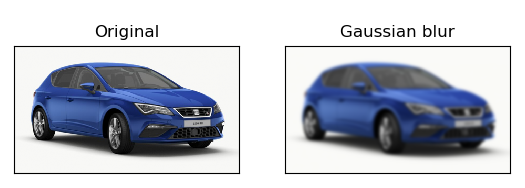
\includegraphics[scale=0.48]{imagenes/blur}
            \caption{aplicación del filtro gaussiano\\ Fuente: Elaboración propia}
        \end{figure}
        % {\centering Fuente: Elaboración propia\par}
        \subsubsection{DETECCIÓN DE BORDES}
        Un borde es esencialmente un cambio brusco de intensidad de los valores de los píxeles en una sección de una imagen, de esta manera, para detectar bordes debemos aplicar algún tipo de suma ponderada que dé como resultado un valor alto si existe un cambio brusco de intensidad, y un valor bajo en caso contrario. 
        Es bajo esta premisa que se propone el filtro Sobel \citep{sobel}, usado luego de aplicar un difuminado gaussiano, y consiste en una combinación entre una convolución gaussiana
        $$\mathcal{G} = \begin{bmatrix}
                                    1\\
                                    2\\
                                    1
                        \end{bmatrix}$$
        \noindent y una aproximación de la derivada parcial de la imagen en espacio discreto con $\Delta_x = \Delta_y = 1$ en cada dimensión
        
        $$\frac{\partial I_{x, y}}{\partial x} = \frac{I_{x+\Delta_x, y} - I_{x-\Delta_x, y}}{\Delta_x}$$
        
        $$\frac{\partial I_{x, y}}{\partial y} = \frac{I_{x, y+\Delta_y} - I_{x, y-\Delta_y}}{\Delta_y}$$
        
        \noindent dando como filtro unidimensional
        
        $$\mathcal{D} = \begin{bmatrix}
                                    1 & 0 & -1
                        \end{bmatrix}$$
                        
        \noindent combinando ambos filtros unidimensionales obtenemos el filtro Sobel para cada dimensión
        \begin{equation}
        \begin{aligned}
        S_x &=  \begin{bmatrix}
                 1\\
                 2\\
                 1
                 \end{bmatrix}
                 \begin{bmatrix}
                 1 & 0 & -1
                 \end{bmatrix}=
                 \begin{bmatrix}
                 1 &  0 &  -1\\
                 2 &  0 &  -2\\
                 1 &  0 &  -1\\
                 \end{bmatrix}\\
        S_y &=  \begin{bmatrix}
                 1\\
                 0\\
                 -1
                 \end{bmatrix}
                 \begin{bmatrix}
                 1 & 2 & 1
                 \end{bmatrix}=
                 \begin{bmatrix}
                 1 &  2 &  1\\
                 0 &  0 &  0\\
                 -1 &  -2 &  -1\\
                 \end{bmatrix}
        \end{aligned}
        \end{equation}
        
        \noindent al ser esta la derivada parcial con respecto de cada dirección, podemos calcular la magnitud mediante la norma $L_2$
        
        \begin{equation}
            \nabla I_{x, y} = \sqrt{S_x^2 + S_y^2}
        \end{equation}
        
        \noindent y la dirección del gradiente
        
        \begin{equation}
            \theta = tan^{-1}\left(\frac{S_y}{S_x}\right)
        \end{equation}
        
        \begin{figure}[H]
            \centering
            % 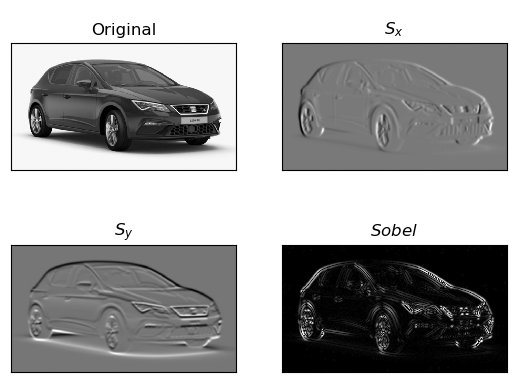
\includegraphics[scale=0.5]{imagenes/sobel_filters}
            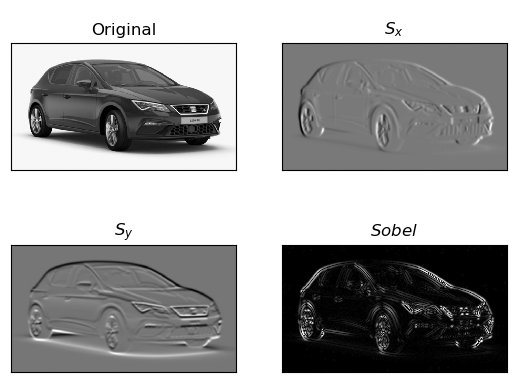
\includegraphics[scale=0.47]{imagenes/sobel_filters}
            \caption{filtro Sobel por dimensiones y total\\ Fuente: Elaboración propia}
        \end{figure}
        % \vspace{-8mm}
        % \begin{center}
        %     Fuente: Elaboración propia
        % \end{center}
        \subsubsection{FILTRO CANNY}
        Los bordes detectados por el filtro Sobel no son independientes de la resolución, por lo que pueden ser más gruesos o delgados dependiendo de la imagen, y detectar como bordes transiciones de iluminación que no lo son necesariamente, es con el fin de refinar este resultado que propone el filtro Canny, que se aplica a la salida de un filtro Sobel \citep{canny}.
        Para aplicar este filtro primero se redondean las direcciones a múltiplos de $45^\circ$ y se procede a verificar si comparado con los píxeles vecinos en esa sección y esa orientación, es el valor máximo o no, en caso que no lo fuese se anula el valor del píxel volviéndolo $0$, caso contrario se continúa con el paso de probar límites de valores, dónde se eligen dos valores $t_{alto}$ y $t_{bajo}$, si un píxel cumple $I_{x,y} \ge t_{alto}$ entonces se considera borde, entonces se verifica cuáles de los 8 píxeles vecinos cumplen $I_{x\pm 1, y \pm 1} \ge t_{bajo}$, finalmente los píxeles que cumplan esta condición se marcan con el máximo valor de un píxel, $255$ y se repite el procedimiento. Si no se cumple la primera condición con el límite alto se asigna el valor $0$ al píxel, obteniendo así una imagen binaria donde los píxeles que representan un borde son de color blanco y los que no, son negros.
        
        \begin{figure}[H]
            \centering
            % 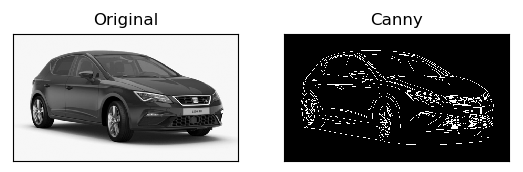
\includegraphics[scale=0.7]{imagenes/canny}
            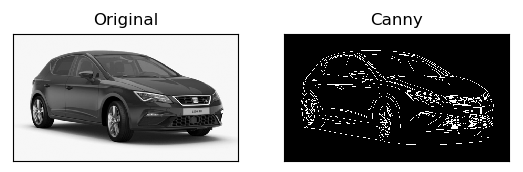
\includegraphics[scale=0.55]{imagenes/canny}
            \caption{aplicación del filtro Canny\\ Fuente: Elaboración propia}
        \end{figure}
        % \vspace{-8mm}
        % \begin{center}
        %     Fuente: Elaboración propia
        % \end{center}
        % \subsubsection{DESCRIPTORES}
        % \subsubsection{CLASIFICACIÓN DE IMÁGENES}
    % \subsection{DETECCIÓN DE OBJETOS}
    % \subsection{SEGMENTACIÓN SEMÁNTICA}

\section{APRENDIZAJE AUTOMÁTICO}
    Del inglés Machine Learning, son métodos basados en la experiencia (datos) que aprenden características de la información disponible para realizar predicciones acertadas \citep{10.5555/3360093}.
    \subsection{APRENDIZAJE SUPERVISADO}
        Es un tipo de tarea de aprendizaje que consiste en extraer características representativas de un conjunto de datos $\mathcal{D}$ y obtener algún mapeo de cada observación $x_i$ a su correspondiente $y_i$, dónde conocemos los $y_i$.
    
        \subsubsection{APRENDIZAJE CORRECTO PROBABLEMENTE APROXIMADO}
        En una tarea de aprendizaje supervisado tenemos un conjunto de datos $\mathcal{D}$ el cual sigue una distribución conjunta
        
        $$\mathcal{D} \sim P(x, y)$$
        
        \noindent con $\mathbf{X}$ el conjunto de observaciones y $\mathbf{Y}$ las etiquetas o valores a predecir. La distribución de los datos es desconocida, por lo que se considera a $\mathcal{D}$ como una muestra aleatoria de tamaño $m$ proveniente de esta distribución.
        
        Con el fin de poder modelar estos datos y aproximarnos a la distribución original para poder realizar inferencias, definimos una función predictiva
        
        $$f: \mathbf{X} \mapsto \mathbf{\hat{Y}}$$
        
        \noindent la cual es parte de una familia de funciones o espacio de hipótesis $\mathcal{H}$ definido por un modelo paramétrico, que se ajustan al conjunto de datos con distintos porcentajes de exactitud, dando como salida el valor esperado dado de $y_i \in \mathbf{Y}$ dado $x_i \in \mathbf{X}$.
        
        $$\hat{y}_i = E(y_i|x_i) = f(x_i)$$
        
        La tarea de aprender consiste en elegir la mejor función $f^* \in \mathcal{H}$, que minimice la esperanza de una función de pérdida $\mathcal{L}(\hat{y}_i, y_i)$. Esta función es una métrica definida en $\mathbb{R}$ que nos permite medir cuán lejos está nuestra predicción $\hat{y}_i$ de un valor esperado conocido $y_i$.
        
        Para obtener la función objetivo se minimiza el riesgo:
        
        \begin{equation}
        \begin{aligned}
            f^* &= \underset{f \in \mathcal{H}}{\text{argmin}} \text{ } E\left[\mathcal{L}(f(\mathbf{X}), \mathbf{Y})\right]\\
            &= \int_\mathbf{X} \mathcal{L}(f(x_i), y_i)dP(\mathbf{X}, \mathbf{Y})
        \end{aligned}
        \end{equation}
        
        \noindent sin embargo no es posible calcular esta integral ya que no se conoce la distribución, por lo que se minimiza el riesgo empírico
        
        \begin{equation}
            \hat{f} = \underset{f \in \mathcal{H}}{\text{argmin}} \frac{1}{m} \sum_{i=1}^m \mathcal{L}(f(x_i), y_i)
        \end{equation}
        
        \noindent el cual también se conoce como función de costo. \citep{10.5555/3360093}
        
    \subsection{REGRESIÓN}
        Uno de los tipos más importantes de tareas de aprendizaje automático es la regresión, en que la variable respuesta es continua, es decir $y_i \in \mathbb{R}$.
        \subsubsection{REGRESIÓN LINEAL}
        Es un modelo que estudia la correlación lineal entre las variables predictoras y las variables predichas, de manera que ajusta el mejor hiperplano (en el caso bidimensional la mejor línea), que modele la correlación lineal de los datos. \citep{gujarati2003basic}
        
        El modelo de regresión lineal se define como:
        
        \begin{equation}
            \mathrm{y}_i = \mathbf{\theta}\cdot\mathbf{x}_i + \varepsilon_i = \theta_0 + \theta_1\mathrm{x}_{i1} + \dots + \theta_n\mathrm{x}_{i n} + \varepsilon_i
        \end{equation}
        
        dónde $\mathrm{x}_{i j}$ es una entrada de la matriz de regresores $\mathbf{X}$ con $m$ observaciones y $n$ características, en la cual el índice $i$ representa el número de observación y $j$ el número de característica para esa observación, $\theta_j$ es un parámetro correspondiente a la $j$-ésima característica el cual representa el grado de incidencia que tiene este atributo sobre la predicción y $\varepsilon_i$: es un término de error que no podemos explicar con las características de nuestros datos o variables regresoras.
        
        \noindent De esta manera se puede reescribir el modelo de manera matricial como:
        
        \begin{equation}
            \mathbf{y} = \mathbf{X}\cdot\mathbf{\theta} + \mathbf{\varepsilon}\label{eq:3}
        \end{equation}
        
        \noindent con
        
        $$\mathbf{X} = \begin{bmatrix}
                        1 & x_{11} & x_{12} & \dots & x_{1n}\\
                        1 & x_{21} & x_{22} & \dots & x_{2n}\\
                        \vdots & & & \ddots & \\
                        1 & x_{m1} & x_{m2} & \dots & x_{mn}\\
                        \end{bmatrix}$$
        
        \noindent y los parámetros
        
        $$\theta = \begin{bmatrix}
                    \theta_0\\
                    \theta_1\\
                    \vdots\\
                    \theta_n
                    \end{bmatrix}$$
                    
        \noindent con función predictora
        
        \begin{equation}
            \mathbf{\hat{Y}} = f(\mathbf{X}) = \mathbf{X}\cdot\mathbf{\theta}
        \end{equation}
        
        Los parámetros $\theta$ que nos permiten encontrar la función $\hat{f}$ se estiman mediante el método de mínimos cuadrados con función de pérdida $\mathcal{L} =  (\mathrm{y}_i - \mathrm{\hat{y}}_i)^2$, y función de costo
        
        \begin{equation}
            E(\theta) = \frac{1}{m} (\mathrm{y}_i - \mathrm{\hat{y}}_i)^2 = \frac{1}{m} (\mathbf{y} - \mathbf{\hat{y}})^\prime\cdot (\mathbf{y} - \mathbf{\hat{y}})
        \end{equation}
        
        \noindent dónde el apostrofe representa la operación de trasposición para el caso matricial.
        
        Desarrollando esta fórmula, derivando e igualando a 0 para encontrar el mínimo, obtenemos una fórmula para calcular los parámetros
        
        \begin{equation}
            \hat{\theta} = (\mathbf{X}^\prime\cdot\mathbf{X})^{-1}\cdot\mathbf{X}^\prime\cdot\mathbf{y}
        \end{equation}
        
        \noindent es así como se obtiene la mejor función predictora estimada $\hat{f} = \mathbf{X}\cdot\hat{\theta}$.
        
        \begin{figure}[H]
            \centering
            % 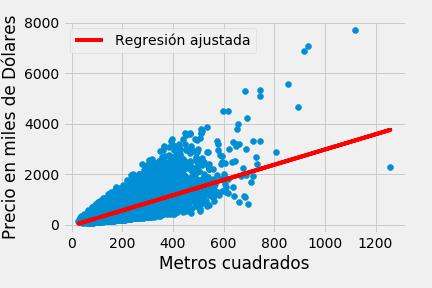
\includegraphics[scale=0.6]{imagenes/linear_fit}
            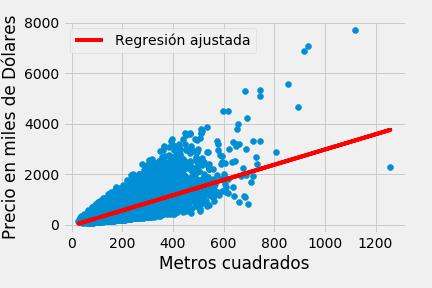
\includegraphics[scale=0.5]{imagenes/linear_fit}
            \caption{Ajuste de una regresión lineal a un conjunto de datos de precios de casas\\ Fuente: Elaboración propia}
        \end{figure}
        % \vspace{-8mm}
        % \begin{center}
        %     Fuente: Elaboración propia
        % \end{center}
    \subsection{CLASIFICACIÓN}
        Cuando la variable respuesta es de tipo categórica, se considera una tarea de clasificación, en que dado un vector de entrada $\mathrm{x_i}$ se debe predecir cuál es la categoría a la que pertenece. \citep{hastie01statisticallearning}
        \subsubsection{REGRESIÓN SOFTMAX}
        Es un modelo lineal generalizado, el cual extiende la idea de la regresión lineal mediante la función de enlace logit multinomial, también llamada softmax, la cual es una generalización de la función sigmoide a múltiples clases, cuyo valor de salida es un vector de probabilidades excluyentes para cada fila de la matriz $\hat{Y}$
        
        \begin{equation}
            Softmax(Z) = \frac{e^{Z}}{\sum_{j=1}^{C} e^{Z_j}}
        \end{equation}
        
        \noindent dónde $Z = \mathbf{X}\cdot\theta$, con $\theta$ ahora de dimensiones $(n \times c)$ siendo $c$ el número de clases, de este modo, mientras mayor el valor de $Z_{i,j}$, mayor es la probabilidad al predecir la clase $j$. \citep{Goodfellow-et-al-2016}
        
        Gráficamente, se interpreta este modelo como el mejor hiperplano que separa el espacio en $c$ partes, donde cada parte contiene las observaciones de su correspondiente clase.
        
        \begin{figure}[H]
            \centering
            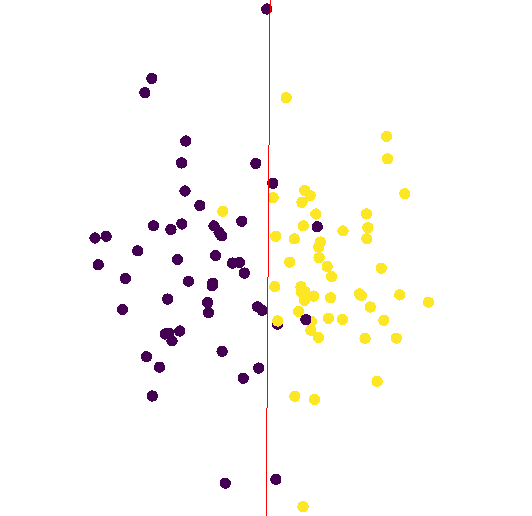
\includegraphics[scale=0.5]{imagenes/logistic_reg}
            \caption{Ajuste de una regresión logística a un conjunto de datos con 2 clases\\ Fuente: Elaboración propia}
        \end{figure}
        % \vspace{-8mm}
        % \begin{center}
        %     Fuente: Elaboración propia
        % \end{center}
        Debido a la nolinealidad de la función de enlace, los parámetros ya no se pueden estimar de manera analítica, por lo que se debe usar un método iterativo para resolver el sistema, sin embargo, lo más importante y requisito de todos los métodos, es encontrar la derivada de la función de costo con respecto a los parámetros.
        
        Con el fin de tener una mejor medida del error para las probabilidades de las categorías, se usa la función log softmax
        
        \begin{equation}
            \mathcal{L} = -log(\hat{y})
        \end{equation}
        
        \noindent derivando por regla de la cadena $\frac{\partial\mathcal{L}}{\partial \theta} = \frac{\partial\mathcal{L}}{\partial Z} \cdot \frac{\partial Z}{\partial \theta}$, obtenemos
        
        \begin{equation}
            \frac{\partial\mathcal{L}}{\partial \theta} = X' \cdot (\mathbf{\hat{y}} - \mathbf{y})
        \end{equation}
        
        \noindent la derivada requisito para cualquier algoritmo de optimización.
        
    \subsection{DESCENSO DEL GRADIENTE ESTOCÁSTICO}
        Uno de los métodos más utilizados para resolver el sistema y encontrar los parámetros de modelos no lineales. Consiste en particionar el conjunto de datos en pequeños lotes, de modo que en cada iteración, se evalúa la derivada en cada lote y se mueven los valores de los parámetros en dirección al mínimo de la función \citep{hastie01statisticallearning}.
        
        \begin{figure}[H]
            \centering
            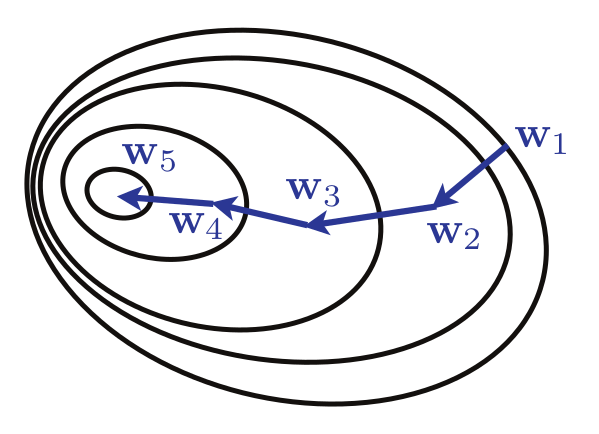
\includegraphics[scale=0.3]{imagenes/sgd}
            \caption{Pasos de los parámetros $W$ en cada iteración camino al mínimo error\\ Fuente: \citep{10.5555/3360093}}
        \end{figure}
        % \vspace{-8mm}
        % \begin{center}
        %     Fuente: \citep{10.5555/3360093}
        % \end{center}    
        {\setstretch{1.0}
        \begin{algorithm}[H]
        	\caption{\textit{Descenso del Gradiente estocástico}}
        	\SetAlgoLined
        	\KwData{$\mathbf{X}:$ Matriz de observaciones}
        	\KwData{$\mathbf{Y}:$ Vector de valores a predecir}
        	\KwData{$\alpha:$ Tamaño del paso de aprendizaje}
        	\KwData{$b:$ Tamaño del lote}
        	\KwData{$f(\mathbf{X}, \theta):$ Función objetivo a optimizar}
        	Inicializar aleatoriamente $\mathbf{\theta}$\\
        	\While{$\mathbf{\theta}$ no converge}{
        		\For{$i$ $\to$ $\frac{m}{b}$}{
        		    $\mathbf{\theta} \leftarrow \mathbf{\theta} - \alpha\cdot \frac{\partial\mathcal{L}}{\partial \theta}_i$
        		}
        	}
        	\Return $\theta$
        \end{algorithm}
        }
        
        \noindent dónde $\mathbf{\theta} \leftarrow \mathbf{\theta} - \alpha\cdot \frac{\partial\mathcal{L}}{\partial \theta}_i$ es la derivada en cada lote.
    
\section{APRENDIZAJE PROFUNDO}
    Buscando resolver el problema de la generalización e invarianza a los datos de los que sufren muchos modelos de machine learning o aprendizaje automático, es que nace el Deep Learning o aprendizaje profundo el cual propone apilar múltiples capas con varias neuronas cada una en una red neuronal para lograr representar funciones más complejas y altamente no lineales, a cambio de requerir muchos más datos para su entrenamiento. \citep{Goodfellow-et-al-2016}
    \subsection{PERCEPTRÓN MULTICAPA}
        El perceptrón multicapa, más conocido como red neuronale, extiende la idea de la regresión logística y lineal a un modelo de $n$-etapas, una especie de concatenación de regresiones con la diferencia que a la salida de las capas se les aplica una función $g(\mathbf{X})$ denominada función de activación, que consiste en alguna transformación no lineal de las variables de salida intermedias con el fin de poder realizar ajustes más complejos a los datos. \citep{hastie01statisticallearning}
        
        \begin{figure}[h]
            \centering
            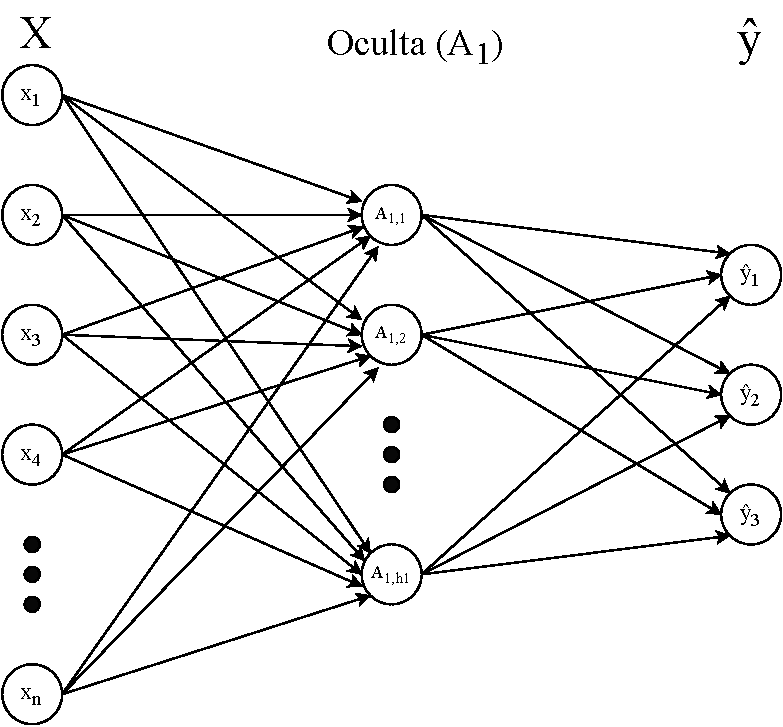
\includegraphics[scale=0.55]{imagenes/NeuralNetwork}
            \caption{Red neuronal con una capa oculta\\Fuente: elaboración propia}
        \end{figure}
        % \vspace{-8mm}
        % \begin{center}
            % Fuente: elaboración propia
        % \end{center}  
        
        Conforme aumentamos la cantidad de capas y parámetros de una red neuronal, esta puede aproximar funciones cada vez más complejas, por lo que se le denomina un aproximador universal de funciones, ya que el espacio $\mathcal{H}$ de todas las posibles funciones que puede aproximar, es infinito, es debido a esto que se requieren más observaciones en la muestra de la distribución de datos a modelar. \citep{Goodfellow-et-al-2016}
        
        La red neuronal matemáticamente es una composición de $n$ funciones o capas, aplicando una no linealidad $g(\mathbf{X})$ en cada etapa, con una función de enlace $g(\mathbf{X})$ en la capa de salida, la cual comúnmente es una softmax para clasificación o la identidad para regresión, siendo esta última etapa una regresión logística o lineal respectivamente, con variables de entrada procesadas por las anteriores capas de manera que sea linealmente aproximable en un número arbitrario de dimensiones elegidas por el modelo al entrenarse sobre los datos. La función de costo se denota por $J(\theta)$ con $\theta$ todos los parámetros del modelo. \citep{bishop}
        
        \begin{equation}
        \begin{aligned}
            Z_1 &= X \cdot W_1 + b_1\\
    		A_1 &= g_1(Z_1) \\
    		Z_2 &= A_1 \cdot W_2 + b_2 \\
    		A_2 &= g_2(Z_2) \\
    		&\vdots\\
    		Z_n &= A_{n-1} \cdot W_n + b_n\\
    		\hat{Y} &= h(Z_n) \\
    		J(\theta) &= \sum_{i}^{m} \mathcal{L}(\hat{y_i}, y_i)
        \end{aligned}
        \end{equation}
        
        Basándonos en la definición de la matriz $\mathbf{X}$ descrita en el modelo de regresión lineal, la columna de unos agregada antes de ajustar el modelo para el parámetro constante, ahora se considerará como un vector de parámetros $b_k$ para las $l_k$ neuronas de la capa $k$, y los demás parámetros son representados por la matriz $W_k$.
        
        \subsubsection{FUNCIONES DE ACTIVACIÓN}
        Con el fin de obtener aproximaciones no lineales a los datos, se debe evaluar la salida $Z_k$ de cada capa en una función de activación no lineal $g_k(Z_k)$.
        
        Las funciones de activación más comúnmente usada por ser fácil de computar y diferenciar es la \textit{Rectified Linear Unit} o \textbf{RELU} \citep{Goodfellow-et-al-2016}, la cual está definida por:
        \begin{equation}
            g(Z_k) = max(0, Z_k) \text{ $\forall$ $z_{k,j}$ / $j$ : $0, 1, ..., l_k$}
        \end{equation}
        
        \noindent cuya derivada con fines de estabilidad numérica es
        
        \begin{equation}
			\frac{\partial g(Z_k)}{\partial Z_k} = 
			\begin{cases}
			\text{1 si } z_{k,j} > 0\\
			\text{0 en otro caso}
			\end{cases}
		\end{equation}
        
        \subsubsection{RETROPROPAGACIÓN DE LOS ERRORES}
        Para ajustar los parámetros o entrenar la red neuronal, al tener más capas por las que pasar para obtener todos los gradientes de los errores, debemos derivar a través de cada una de ellas, a este algoritmo se le llama Backpropagation o Retropropagación, que es simplemente como su nombre dice, propagar los gradientes de reverso a través de la red neuronal.
		
		Primero se obtiene la derivada con respecto da cada uno de los parámetros de la composición de funciones por regla de la cadena
		
		\begin{equation}
		    \frac{\partial J}{\partial \theta_k} = \frac{\partial J}{\partial Z_n} \cdot  \frac{\partial Z_{n}}{\partial A_{n-1}} \cdot \frac{\partial A_{n-1}}{\partial Z_{n-1}} \cdot  \dots \cdot \frac{\partial A_{k}}{\partial Z_{k}} \cdot \frac{\partial Z_{k}}{\partial \theta_{k}}
		\end{equation}
		
		\noindent dónde $\theta_k$ representa cualquiera de los parámetros de $W_k$ o $b_k$ en la capa $k$, notese que para obtener la derivada con respecto de los parámetros en la capa $k$ se requiere la derivada en con respecto de las activaciones las capas siguientes, así, cuando obtenemos la derivada con respecto de los parámetros de la capa $k$ ya calculamos para todas las capas siguientes y sólo debemos multiplicar por la derivada de la salida lineal de la capa $k$ con respecto del parámetro $\theta_k$. \citep{bishop}
		
		Para el caso de regresión y clasificación con softmax $\frac{\partial J}{\partial Z_n} = (\mathbf{\hat{Y}} - \mathbf{Y})$ de forma vectorial, de manera general la derivada con respecto de algún parámetro está dada por
		
		\begin{equation}
		    \frac{\partial J}{\partial \theta_k} = \frac{\partial J}{\partial Z_n} \cdot \prod_{i=0}^{n-(k+1)} W_{n-i} \frac{\partial g_{n-(i+1)}(Z_{n-(i+1)})}{\partial Z_{n-(i+1)}} \cdot \frac{\partial Z_k}{\partial \theta_k}
		\end{equation}
		
		Similar a la regresión logística, se estiman los parámetros mediante un método de optimización, cuyo requisito sea la derivada con respecto a cada uno de los parámetros.
		
    \subsection{REDES NEURONALES CONVOLUCIONALES}
        Es un tipo de arquitectura de redes neuronales diseñada específicamente para tareas sobre imágenes, de manera que las operaciones sobre las observaciones de entrada ya no son composiciones realizando multiplicaciones matriciales, sino que cada neurona se convierte en un filtro o kernel de dimensiones $(k \times k)$, de los cuales tenemos varios filtros que se aplican sobre la imagen mediante la convolución.
        
        \begin{figure}[H]
            \centering
            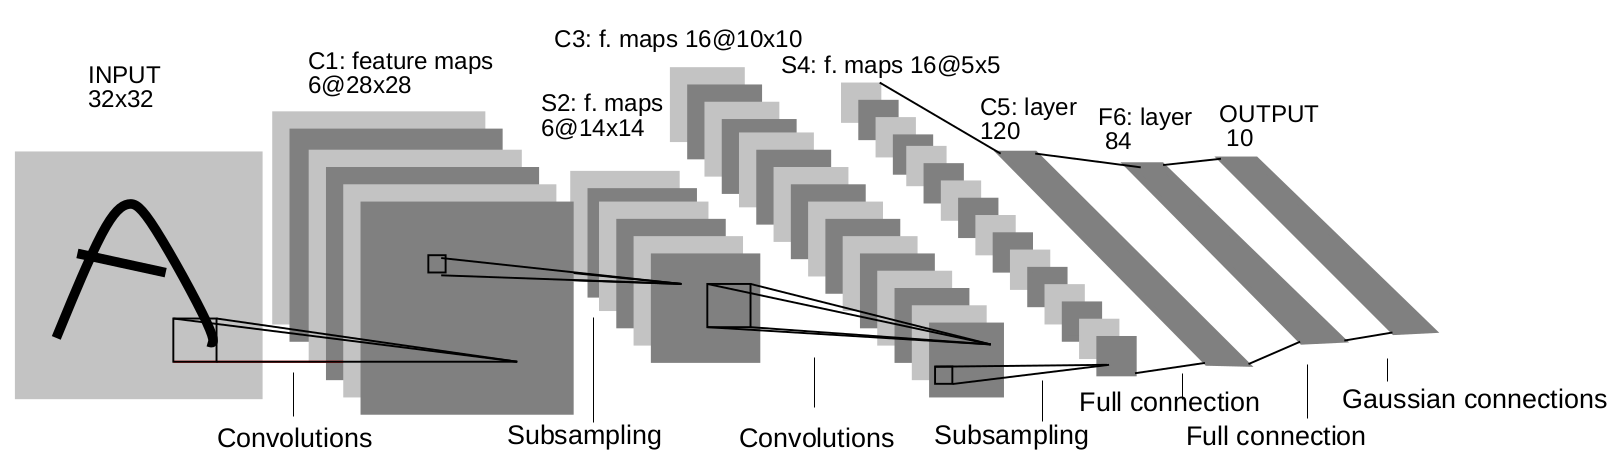
\includegraphics[scale=0.25]{imagenes/lenet}
            \caption{Red neuronal convolucional para la clasificación de dígitos manuscritos\\ Fuente: \citep{lecun-gradientbased-learning-applied-1998}}
        \end{figure}
        % \vspace{-8mm}
        % \begin{center}
        %     Fuente: \citep{lecun-gradientbased-learning-applied-1998}
        % \end{center}
        La idea detrás de este tipo de red es que se apliquen varios filtros en cada capa de la red para extraer características importantes de los objetos que se buscan, estos filtros se aprenden mediante retropropagación y ya no se diseñan a mano \citep{Goodfellow-et-al-2016}.
        \subsubsection{STRIDES}
        Cuando se desea optimizar la operación sacrificando representabilidad o disminuir la muestra, se puede incrementar el tamaño del salto de la ventana deslizante al convolucionar la imágen con el filtro, a este salto se le llama \textbf{stride}
        
        
        Aplicando esta idea, se obtiene una fórmula general para calcular la dimensión de la matriz resultante al aplicar cada uno de los filtros con un stride $s$
        
        $$\frac{I_{alto} - k + s}{s} \times \frac{I_{ancho} - k + s}{s}$$ 
        
        \begin{figure}[H]
            \centering
            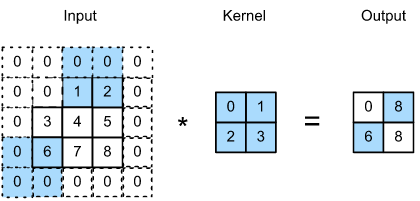
\includegraphics[scale=0.6]{imagenes/stride}
            \caption{Convolución con $s=2$\\ Fuente: \citep{zhang2020dive}}
        \end{figure}
        % \vspace{-8mm}
        % \begin{center}
        %     Fuente: \citep{zhang2020dive}
        % \end{center}
        \subsubsection{POOLING}
        Es una operación sobre la entrada bidimensional que con un stride $s$ recorre una ventana deslizante de dimensión $p \times p$ extrayendo información característica de cada sección de la entrada.
        
        Existen dos tipos de pooling más comunes, average pooling que promedia los valores activados en cada sección de la imágen sobre la que pasa la ventana y max pooling, el cual extrae el elemento más representativo, es decir el con mayor valor, de cada sección de la imágen.
        
        \begin{figure}[H]
            \centering
            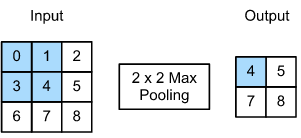
\includegraphics[scale=0.6]{imagenes/pooling}
            \caption{Pooling con con $s=1$\\ Fuente: \citep{zhang2020dive}}
        \end{figure}
        % \vspace{-8mm}
        % \begin{center}
        %     Fuente: \citep{zhang2020dive}
        % \end{center}
    \subsection{APRENDIZAJE DE REPRESENTACIONES PROFUNDAS}
    En cada etapa de la red neuronal se extraen características representativas de la imagen que ayuden a realizar la predicción de la tarea para la cual se la entrena, conforme pasan más etapas en la red los filtros buscan características más específicas \citep{Goodfellow-et-al-2016}
    
    \begin{figure}[H]
            \centering
            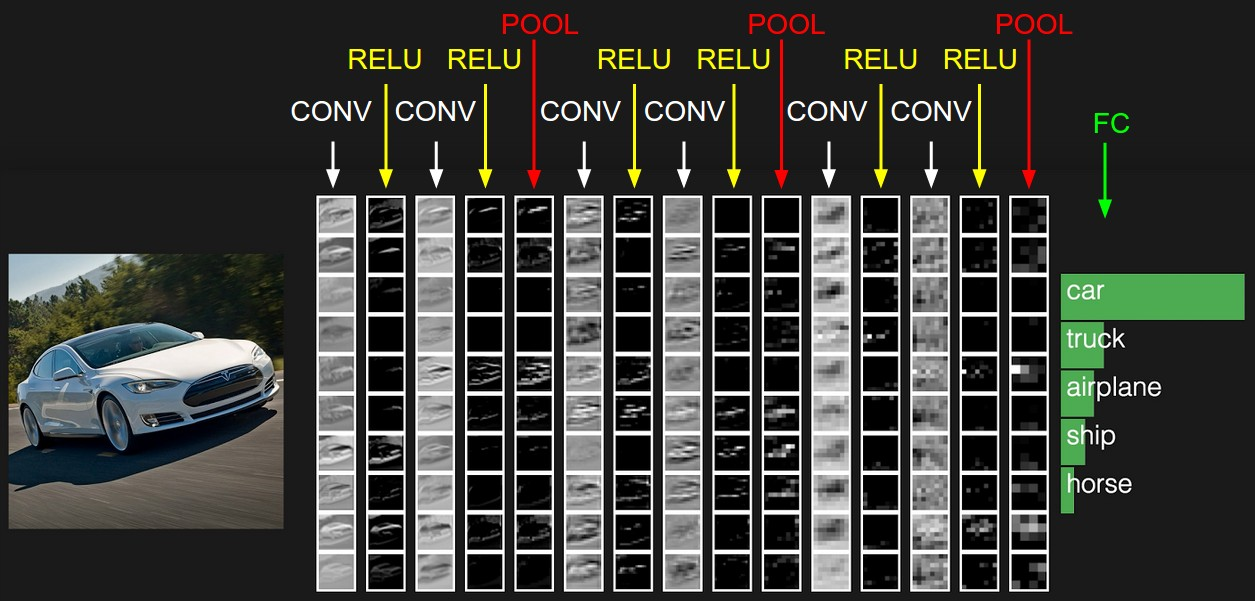
\includegraphics[scale=0.3]{imagenes/convnet}
            \caption{Extracción de las características profundas aprendidas\\ Fuente: \citep{stanford_2020}}
        \end{figure}
        % \vspace{-8mm}
        % \begin{center}
        %     Fuente: \citep{stanford_2020}
        % \end{center}
    
    \noindent de esta manera activando (dando valores altos) a ciertas partes de la imagen que es donde ``presta atención'' en busca de los objetos que desee clasificar o en base a los que predecir algún valor numérico

    \begin{figure}[H]
            \centering
            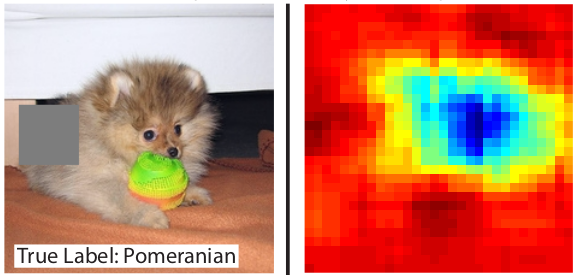
\includegraphics[scale=0.5]{imagenes/activation_cnn}
            \caption{Activación de los píxeles de la imagen en la $5^{ta}$ capa de la red\\ Fuente: \citep{10.1007/978-3-319-10590-1_53}}
        \end{figure}
        % \vspace{-8mm}
        % \begin{center}
        %     Fuente: \citep{10.1007/978-3-319-10590-1_53}
        % \end{center}
    \noindent a esto se le llama aprendizaje de representaciones profundas, porque los filtros aprenden información desde bajo a alto nivel que caracterice los objetos en las etiquetas de entrenamiento. 